\chapter{Fonctionnement et Tests}

Dans cette partie nous allons tout d'abord nous pencher sur le fonctionnement et les tests concernant la partie parser du projet, puis nous allons aborder les mêmes points pour la partie analyse des données.

\section{Parser}

Cette partie du projet est écrite en java, nous avons utilisé JUnit afin de mener à bien ces tests unitaires. De plus le dépôt git est muni d'un outil d'intégration continue (Travis) qui est assoscié à nos tests afin de garantir que le développement ne produit pas d'erreurs sur le fonctionnement du programme. \\

De plus nous avons effectué des tests de couverture en utilisant le plugin Cobertura Maven qui nous a aidé à détecter les points plus faibles au niveau des tests et ainsi proposer d'autres tests unitaires pour avoir une meilleur couverture.


\subsection{Politique de tests}

Du fait de l'utilisation de java, pour chaque classe non-utilitaire un premier test vérifie systématiquement que la création des objets fonctionne correctement, une fois ce critère validé, des tests spécifiques à chaque classe sont effectués en fonction des fonctionnalités qu'elles remplissent.\\

Le but de nos test est de verifier l'extraction des donnéees des logs, pour cela, nous avons choisi deux logs réels représentatifs de chaque version et avons appliqué la stratégie suivante:  \\
En premier lieu nous avons réalisé des test pour verifier la bonne detection de la version pour les différents types de version. \\
Ensuite nous avons pris chaque donnée de la structure et avons validé qu'elle ne soit pas vide, dans le cas où l'élément est une liste, nous vérifions que le nombre d'éléments correspond, et finalement pour les éléments carte/quantité, comme par exemple \textit{victory cards} ou \textit{market} nous vérifions que le couple nom, valeur corresponde.

\subsection{Tests unitaires}

Les tests proposes pour la validation du module Java sont faites avec des logs réeeles et sans aucune altération.\\
On a disposé de six logs, deux représentafs de chaque type de version. \\

Dans la class LogReaderFactoryTest, on voulait tester la lecture du log, la creation du object LogReader qui instance la version correspondant et la construction du object Document complet avec tous les donnéées du log pour envoyer au base de données. \\

Dans les class LogReaderV1HeaderTest, LogReaderV2HeaderTest et LogReaderV3HeaderTest, on rendre en le détail du object Document, et on analyse que les attributes Date, name, Winners, Cards Gonne, cards Market et cards Trash soient corrects en nom, nombre et quantite a ce-lui qui on trouve dans les logs. \\

Dans la class LogReaderPlayerTest on valide les données propres du joueur, pour les test on utilise trois log, un de chaque version et pendant les preuves on prend un joueur different au hasard de chaque log. On verifie que le nombre de joueur du object corresponde ou nombre du log, les noms des joueur, les nombre points et les nombre de turns. \\
Pour les données de Cards Victory, cards Deck, Cards FirstHand et Cards Opening on valide nombre, nom et quantite. \\

Finalement la class PlayerTest qui verifie la conection avec la base de donnée et la pas duplication de Joueurs avec le même nom.

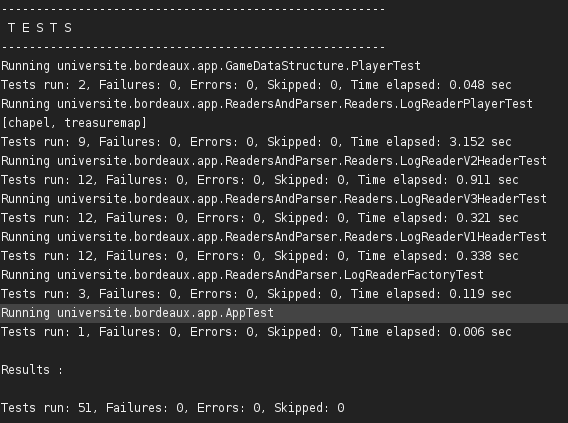
\includegraphics[scale=0.35,keepaspectratio]{./unit_tests_jave}

Avec un total de 51 test executées, avec aucun erreur ou échec.

\subsection{Tests de couverture}
Voici les resultats obtenus lors des tests de couverture de la partie Parser du projet:

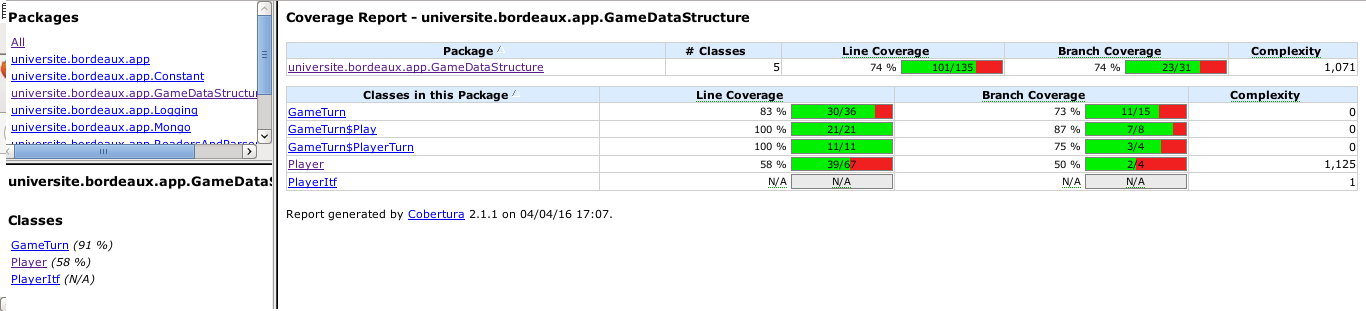
\includegraphics[scale=0.35,keepaspectratio]{./coverage_GameDataStructure}

Dans la partie structure de données n'avons pas testé l'utilisation d'actions successives dans un même tour (combo). L'autre portion de code non testée correspond à la conversion des données d'un joueur contenues dans le serveur vers un objet de type Player, ce cas de figure ne se produit jamais avec l'utilisation que nous faisons de la partie java mais si jamais le projet venait a évoluer et utilise des données de joueurs déja présentes dans le serveur, il faudra effectuer des tests sur cette partie.

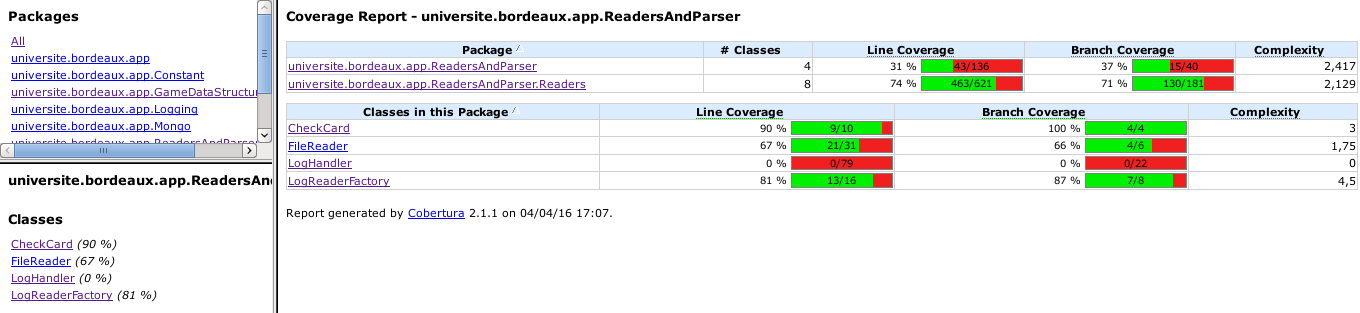
\includegraphics[scale=0.35,keepaspectratio]{./coverage_ReadersAndParser}

Pour la partie préparant le parsing (c'est a dire avant l'utilisation du parser), par manque de temps, nous n'avons pas pu tester le LogHandler. Pour le module FileReader, nous n'avons pas testé les cas aux limites, ce qui entraine la non-couverture des lancement d'exceptions. Pour le module LogReaderFactory, la portion non traitée correspond au cas ou une partie du header d'un log est manquante, il aurrait fallu rajouter un ce cas de figure.

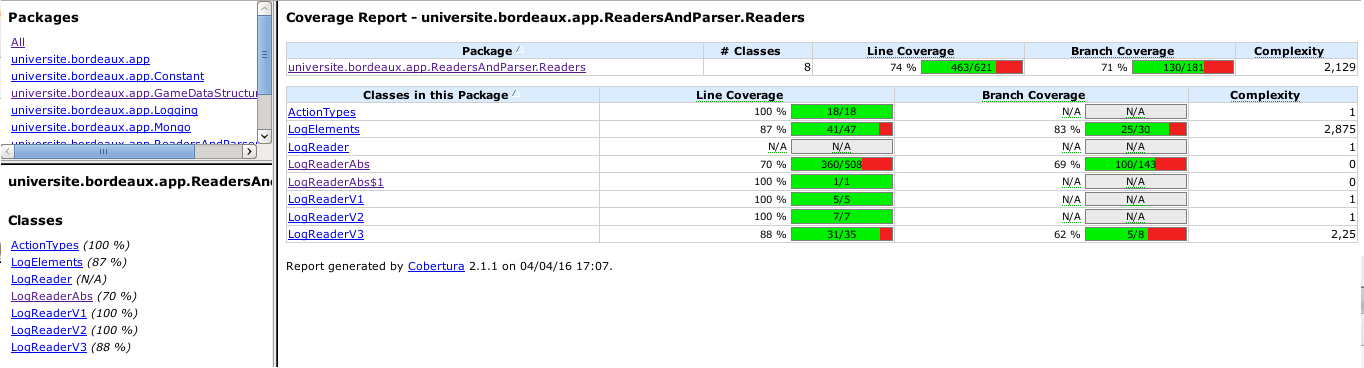
\includegraphics[scale=0.35,keepaspectratio]{./coverage_ReadersLog}

Pour le module LogReaderAbs, nous n'avons pas testé le cas de figure ou plusieurs joueurs gagnent à ex-aequo. Le reste du code non couvert correspond à des cas de figures plus rares, pour obtenir une couverture de ces portions de code, il aurait fallu trouver ou bien construire des logs plus variés. Le temps nous a empêché d'effectuer ce travail assez long.

\section{Bugs rencontrés}

\paragraph*{Dictionnaire de Cartes} 

Il existe une classe qui sert à verifier l'existence d'une carte et returne en même temps le nom générique de la carte donnée.\\
Il y a des problèmes avec les cartes dont le pluriel change radicalement du singulier. par exemple les cartes Colonies (Colony) et Duchies (Duchy). \\

Pour resoudre le bug il faut changer le dictionaire actuelmement implementé, pour ajouter la convertion de cartes en pluriel qui sont des cas atypiques.

Pour la classe logReaderAbs, il y a des actions qui ne sont pas testées car, dans les logs selectionnés pour les tests il n'existe pas toutes les actions possibles pour les Joueurs, une solution serait de modifier le .

\paragraph*{Nom de Joueurs} 

Dans les logs nous avons trouvé des noms de joueurs très dificiles à traiter car ils ont beaucoup de caractères spéciaux ainsi que des noms explicitement ecrits pour casser des programmes,
par exemple System.out.println("hola"), ou ;) ou même , des noms avec des mots reservés pour les langages de programmation.


\section{Module d'analyse des donnée}
Cette partie du projet écrite en Python est cruciale car c'est ce qui sera utilisé par l'utilisateur. Nous avons utilisé le module unittest pour effectuer nos tests unitaires ainsi que mongomock pour simuler l'utilisation d'un serveur MongoDB. Les tests de couverture ont été effectués à l'aide de pytest

\subsection{Politique de tests}
Nous avons testé le module Match et Tools afin de vérifier leur bon fonctionnement, les tests effectués sont des tests unitaires. Pour effectuer nos tests, nous avons produit un log prédéfini a comparer au résultat des tests effectués.

\subsection{Tests unitaires}
\paragraph{module Match}
Trois tests unitaires ont été effectués:
\begin{itemize}
\item un test de comparaison du nom des joueurs.
\item un test de comparaison du log a proprement parler, c'est à dire les actions des joueurs au cours de la partie
\item un test de comparaison des informations du header.
\end{itemize}

Ces trois tests passent sans poser de problèmes.

\paragraph{Module Tools}
Trois tests unitaires ont été effectués:
\begin{itemize}
\item un premier test permet de vérifier la bonne crétation de la pseudo base de données (utilisation de mongomock).
\item un second test vérifie la bonne création des informations gloabales pour chaque joueur présent dans le log test (2 joueurs).
\item le troisième test vérifie que la fonction de calcul d'elo s'applique correctement ainsi que la détection du \textit{greening}.
\end{itemize}

\subsection{Tests de couverture}
Le résultat des tests de couverture est le suivant:\\
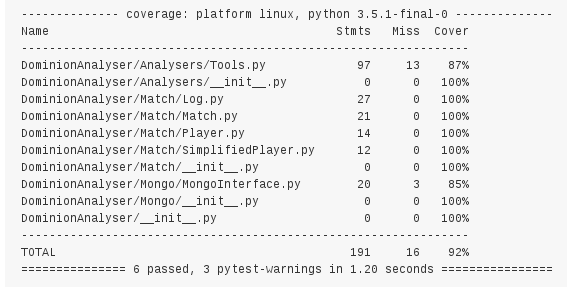
\includegraphics[scale=0.35,keepaspectratio]{./coverage_python_code}
Nous ne couvrons pas totalement le module Tools, cela s'explique par le fait que nous n'avons pas fait de tests sur la reconaissance des stratégies.\\
Le module MongoInterface n'est pas entièrement couvert non plus, car nous ne testons pas la création d'index et de collections.


\paragraph{conclusions}
Par manque de temps, nous n'avons pas pu effectuer plus de tests mais une suite logique à ces quelques tests unitaires serait de produire des logs pouvant poser problème, par exemple avec des caractères spéciaux ou bien des mots clefs relatifs au langage python. Concernant les test unitaires des outils, d'autres tests pourraient être effectués pour la detection des stratégies ou bien pour des valeurs d'ELO ambigües.



\subsection{Bugs rencontrés}
Du fait du peu de tests, nous n'avons pas rencontré de bugs sur ces tests mais les pistes évoquées dans la partie tests de couverture ne manqueront pas de révéler des faiblesses potentielles dans le code produit.

\iffalse
\subsection*{Sous-partie 1 ('apparaitra pas dans l'index)} Bla



\paragraph*{Paragraphe 3} Bla

\newpage

\subsection*{Sous-partie 2}

Bla

%galerie d'image
\begin{figure}[htp]
  \centering
  \subfloat[Première image]{\label{fig:première}
\includegraphics[scale=0.8]{resultats/gallerie}}
  ~ %espace entre deux images sur une même ligne
  \subfloat[Deuxième image]{\label{fig:deuxième}
\includegraphics[scale=0.8]{resultats/gallerie}}
  ~
  \subfloat[Troisième image]{\label{fig:troisième}
\includegraphics[scale=0.8]{resultats/gallerie}}
  ~\\ %saute une ligne dans la galerie d'image
  \subfloat[Quatrième image]{\label{fig:quatrième}
\includegraphics[scale=0.8]{resultats/gallerie}}
  ~
  \subfloat[Cinquième image]{\label{fig:cinquième}
\includegraphics[scale=0.8]{resultats/gallerie}}
  \caption{Différents screenshots quelque chose, en gallerie}
  \label{fig:gallerie1}
\end{figure}
\fi
